\RequirePackage[hyphens]{url}

\documentclass[sigconf]{acmart}

\usepackage{graphicx}
\usepackage{hyperref}
\usepackage{todonotes}

\usepackage{endfloat}
\renewcommand{\efloatseparator}{\mbox{}} % no new page between figures

\usepackage{booktabs} % For formal tables

\settopmatter{printacmref=false} % Removes citation information below abstract
\renewcommand\footnotetextcopyrightpermission[1]{} % removes footnote with conference information in first column
\pagestyle{plain} % removes running headers

\newcommand{\TODO}[1]{\todo[inline]{#1}}

\begin{document}
\title{How Far Have Spacewalks Walked}

\author{Rick Alan Carmickle Jr.}
\affiliation{%
  \institution{Indiana University School of Informatics and Computing}
  \streetaddress{919 E. 10th Street}
  \city{Bloomington} 
  \state{IN} 
  \postcode{47408}
  \country{USA}}
\email{rcarmick@iu.edu}


% The default list of authors is too long for headers}
\renewcommand{\shortauthors}{R. Carmickle}


\begin{abstract}
We use data from the NASA Open Data Portal mission parameters parsed from the Wikipedia pages of manned spaceflight missions of the U.S. and Russian space programs to analyze American and Russian spacewalks. We calculate the distance traveled, relative to the earth's surface, by astronauts and cosmonauts who performed Extravehicular Activities (EVA) in earth orbit. As part of that calculation, numerous other orbital parameters will be calculated. 

\end{abstract}

\keywords{i523, HID304, Big Data, Wikipedia API, Extra Vehicular Activity}

\maketitle


\section{Introduction}
This was an exercise in using datasets from unrelated sources, cleaning that data so that links between datasets could be formed, then creating mathematical analysis and visualizations of the data from necessary elements in these different datasets. The data used was a combination between an existing dataset created by NASA as part of the NASA Open Data initiative, and mission trajectory datasets created by gathering and cleaning data on manned space launches via the Wikipedia API. 

The goal was to measure the distances traveled through space by humans in earth-orbit spacewalk. At the outset, an objective of this project was to create a geovisualization of an orbital ground trace for the specific area spacewalks occurred. The author discovered that several pieces of data necessary to perform the objective were missing from Wikipedia data. This paper will end with a discussion of exactly what data is needed, in addition to what is available here, to create orbital ground traces and highlight portions of those traces.
 
\section{Explanation of Terms}
Terms related to orbital mechanics and the data sources need to be defined at the outset.

Spacewalk and Extravehicular Activity are synonymous. This refers to events when a human in a vessel outside earth's atmosphere leaves the interior or opens the hatch of a vessel exposing the interior to space \cite{Aeronautics1995}. 

The Infobox of a Wikipedia page is the table on many pages with facts and summaries of the article's topic. This is an embedded object on Wikipedia pages with standard syntax but many variations on how it can be used \cite{Wikipedia17}.

The Apogee or Apoapsis of an orbit is the orbit's maximum distance from the body it is orbiting in an elliptical path. Apogee refers specifically to objects in Earth's orbit and Apoapsis is a general term. Perigee or Periapsis of an orbit is the orbit's minimum distance from the body it is orbiting in an elliptical path \cite{Wolfson2007}. Perigee refers specifically to objects in Earth's orbit and Periapsis is the general term. Both of these measurements are typically recorded as distances from the surface of the orbited body \cite{Muirden1982}.

Orbital eccentricity is a measurement of the difference between the apoapsis and periapsis. Put another way, it is a measurement of how elliptical an orbit is. An eccentricity of 0.0 indicates a perfectly circular orbit. An elliptical orbit will have an eccentricity of between 0.0 and 1.0. Eccentricity greater than or equal to 1.0 indicates an escape trajectory \cite{Muirden1982}. 

Orbital inclination is a measurement of the angle between an object's orbital plane and the earth's equatorial plane. An inclination of 0.0 is a perfectly equatorial orbit traveling east relative to the Earth's surface: the same direction as the Earth's rotation. An inclination of 90.0 is a polar orbit and an inclination of 180.0 is a perfectly equatorial orbit traveling west against the Earth's rotation \cite{Muirden1982}. 



\section{Getting the Data}
The starting point is the dataset from the NASA Open Data Portal, a 2015 dataset entitled ``Extra-vehicular Activity (EVA) - US and Russia’’ \cite{NASA2014}.  This dataset contains plaintext of the country, crew, vehicle, duration, and purpose of each spacewalk. The official start of each space walk, defined as the moment an astronaut or cosmonaut has begun exiting an open hatch in a depressurized vessel, is included as a date.

From the ‘Vehicle’ category of this data, a single column of unique mission names was generated manually. This single column was formatted to remove non-mission-related text and appended to a single-category csv file. The 'Vehicle category formatting was vital to this project since this was the merging category for the EVA dataset and orbital parameter dataset.

The Jupyter notebook '1-gathering-wikipedia-infobox-data' contains the steps for creating a dataset with significant details on each given mission which can be generated from the a single category containing the name of the mission. 

The data gathering stage of the project emerged, over the course of this project, as the step with the highest Big Data potential. The usability and flexibility of the code developed here was unexpected for the author and has demonstrated applicability for gathering and parsing Wikipedia data for other desired categories.

Several different open-source libraries were used together at this stage in a notebook capable of identifying and sorting categories of data from JSON templates contained on given Wikipedia pages  \cite{stackoverflowquestions}. This notebook is specific to the categories of interest in this project because the names of the Infobox parameters desired must be specifically given as arguments. 

These parameters could, however, could be altered to fit any set of Infobox categories. The interface for searching and retrieving JSON data on Wikipedia pages was tested during development with wikipedia pages unrelated to manned space travel and is capable of retrieving data from pages with different JSON configurations on data charts contained on Wikipedia. 

The ‘mission-name’ file is the only necessary input file to generate the dataset. The only requirement of the category names in this file is that they must be close to the string that would appear as the title of the desired Wikipedia page. They do not, however, need to be an exact match. The `Wikipedia’ library by Jonathan Goldsmith \cite{Goldsmith2017} is a flexible library which can access the Wikipedia API and utilize Wikipedia’s search function to retrieve the URL of the desired page. This library had many functions for accessing Wikipedia data, but does not include a method to access tables and charts.

This library was capable of identifying than an input of ``Gemini IV’’ corresponds to the proper article title of ``Gemini 4’’ and the exact URL string of ``https://en.wikipedia.org/wiki/Gemini-4’’. The exact article title string is necessary for the step which iterates through individual pages and appends the data.

The data fetching process makes a request through pywikibot \cite{Wikimedia} of the Wikipedia API for a given page. Pywikibot retrieves a raw version of the entire page. Mwparserfromhell \cite{Kurtovic2017} identifies templates matching JSON charts and returns a name and value list for every parameter name and values for every JSON chart template on each page. 

The input file which provides article titles and the category names matched to the parameter names in the JSON date could be changed to retrieve data for other interests. The code uses for gathering the data is not efficient and had much room for improvement. A future project the author will pursue is an interface which accepts a column of strings corresponding to entities with Wikipedia pages and a column of parameter names from the Infobox and returning a dataset which fills as much data as is available. 

\section{Cleaning the Data}
The Jupyter notebook '2-data-cleaning-and-merging' cleans both the EVA and raw mission datasets. The ‘mission-data-raw.csv’ data is not a usable dataset immediately following parsing from Wikipedia. The author was unable to implement code to recognize raw JavaScript and JSON data to append only the necessary substrings, so this textual data was cleaned with code written specifically for each category. This stage relies heavily on basic string editing functions such as replace, strip, and split. For maximum flexibility with calculations, elements of the data were reduced to the simplest components or summarized in a way that left a single integer or floating value. 
For example, the original string scraped from Wikipedia for ‘mission duration’ was roughly formatted as “n months, x, days, y hours, z minutes” but permutations of JavaScript code, misread ASCII characters, and inconsistencies in the categories used were common. Several categories of data were added in the data cleaning process. 
One instance of data creation which should be noted is the appending of current International Space Station (ISS) orbital parameters to all missions beginning with “Expedition”. This data should be considered an experimental stand-in for complete data for respective spacewalks because the ISS’s orbit is not stable. The orbit of the ISS decays over time since the craft experiences a small amount of atmospheric drag \cite{Hutchinson2013}. The ISS is also navigated in orbit. The true orbital parameters of the ISS for the duration of any given spacewalk would require a data framework which can access the orbital history of the ISS, a function beyond the scope of this project and the skillset of the author. The ISS has, however, remained close to 250 miles overhead for the duration of its existence and has never been accelerated to create a high orbital eccentricity, so a generalized set of orbital parameters will provide an acceptable baseline for ISS spacewalks.

The data cleaning for many categories was a repetitive task of removing errant characters. Future development would benefit from the author better understanding the relationship between JavaScript, JSON, html, and Python so that syntax from one language can be cleaned before importing to a data file.

The mission data parsed from Wikipedia was not the only dataset that needed addressing. The EVA dataset required work to render it usable. This dataset included many one-time typos and oddities in columns which required manual changing in the csv data. “Extra-vehicular-Activity--EVA----US-and-Russia.csv” is therefore not exactly as one would find it from the NASA Open Data Portal. The precise alterations made to this data are detailed in  “changelog to Extra-vehicular-Activity--EVA----US-and-Russia.txt”. The altered EVA datafile is needed to run this project. 

New categories of data were generated from the EVA dataset before it was ever merged with the orbital parameter data. The single string of crew names was split into separate columns, each containing either the name of a crew member who participated in EVA or ‘NaN’. The spacewalk duration, in seconds, was calculated for ease in mathematics later on. 
Over the course of this project, the author learned much about orbital ground tracks and was refreshed on the mathematics underlying orbital mechanics. One of the limitations of the EVA dataset was revealed at this stage: The dataset includes the data (month/day/year) where a given spacewalk occurred, but the creation of an orbital EVA ground trace would require the month, day, year, hour, minute, and second of the beginning of an EVA to create an accurate trace given the relative speed over the ground of low-earth orbit spacecraft. The available data does provide information accurate enough to calculate orbital velocity and distances traveled. 

The data cleaning notebook ends with merging the EVA data and the orbital parameter data into a single DataFrame on the ‘Vehicle’ column.

\section{Data Analysis and Calculations}
The third notebook uses only the new dataset ‘spacewalk-with-orbital-data.csv.’ Because the data has been cleaned, merged, and homogenized to consistent units of measurement, the mathematics of further orbital details are relatively simple calculations across a DataFrame.  The Earth’s equatorial radius and gravitational constant \cite{Williams2016} are variables contained within the notebook and units are converted as needed.  
From the data scraped from the Wikipedia API, we can calculate the semi-major and semi-minor axes of each orbit, the eccentricity, and the orbital velocity of a given orbits where all earlier parameters were present \cite{Wolfson2007}. 

\section{Results}
The initial question of "How far have spacewalks walked" is answered with the data generated here, with the caveat that input data is imperfect. The longest single spacewalk, in terms of time spent in EVA and distance traveled relative to the earth, is a 2001 Space Shuttle Mission working on the ISS where Jim Voss and Susan Helms worked outside for 8 hours and 56 minutes and traveled 246,946,540 meters relative to the earth's surface. Table \ref{t:mytable} includes the descriptive EVA data as well as the final calculated fields for the twenty most traveled spacewalks. 

Figure \ref{f:fig1} features the final calculated spacewalk distances for every spacewalk. Only the mission label is included. Repeats of a label indicate multiple EVAs by a mission's crew. The distances traveled range from the roughly 5,500 kilometers traversed by Alexei Leonov over 12 minutes in the very first human spacewalk to the quarter of a million kilometers traveled by Mission Specialists Jim Voss and Susan Helms in their 8 hour and 56 minute spacewalk as part of an early resupply mission to the ISS. 

Figure \ref{f:fig2} is a parallel coordinate plot of the year a given EVA took place mapped to EVA duration.  From this visualization, we see the increasing volume of spacewalks as well as the general increase in EVA time over the years as the technology to sustain low-earth orbit EVAs improved and space program efforts were focused on the construction of the ISS. 

Upon basic exploration of the data, we see some trends by mission type. The most eccentric orbits were often the earliest, with Gemini, Voskhod, and Apollo appearing as the most eccentric. STS and Gemini missions appear to be the missions with the largest orbital perimeters. The highest orbital velocities, directly related to how close to the surface an object orbits, are topped by Soyuz missions from the late 1980s through the early 2000s as well as STS missions. 

A glance at the orbital inclination reveals a distinct pattern in this category. Data points are clumped around the values of 28 and 50. Figure \ref{f:fig3} is a scatterplot of spacewalk duration and orbit inclination, colored by country \cite{Waskom2017}. There is a reason for the distinct clumping in the data along those values.

The inclination of an orbit is a measurement of the object's orbital plane compared to earth's equatorial plane. An orbiting object's inclination can never start at less than the latitude of the launch site. Lowering the inclination of an orbit below the starting latitude requires an adjustment burn at either orbital insertion or during orbit when latitude matches the desired inclination \cite{Davis2012}. In Figure \ref{f:fig3}, the lower line of datapoints, at a value around 28 corresponds to the Latitude of Kennedy Space Center, which is the source of most American launches and is located at 28°28′N 80°32′W. The upper clumping of data points, at a value around 52 corresponds to the ISS inclination of 51.64 degrees. 

The predicted and actual orbital period categories present an opportunity to test the validity of the calculations made with this dataset. We would expect an ideal 1-to-1 relationship between predicted and actual orbital periods. The predicted and actual periods are, in this instance, independent variables since predicted period was calculated with Apoapsis, Periapsis, semimajor axis, and constant values of earth's properties \cite{Wolfson2007,Muirden1982}. The actual orbit period measurement was not part of the calculation. The difference between these values has a mean of 6.265 seconds, a median of 0.210 seconds, and a standard deviation of 38.75. With single columns of mathematically independent variables, a linear regression is appropriate \cite{Community2017}. Figure \ref{f:fig4} displays the results of the linear regression model. The p-value of this model is 1.824 u-150. This is a demonstration of an effective relationship between variables as expected. In this model, the slop and intercept would carry some significance. The ideal relationship between two identical variables should have an intercept of 0 and a slope of 1 \cite{Frost2014}. The intercept of 441.38 is 7.996 percent of the mean of actual orbital periods. The slope of 0.9211 is 7.89 percent less than the expected slope. Both slope and intercept \cite{Frost2014} are almost precisely 8 percent deviated from the ideal expectation R-value and standard error confirm that the calculated orbital period is deviated by approximately 8 percent from the true values reported in the data \cite{Frost2014}. 

The geovisualization aspect of this project ultimately failed. After beginning the process of creating orbital ground traces through BaseMap, it was discovered that a precise ground trace requires some additional data either unavailable or unparsed from the Wikipedia data. A ground tracing function would require the time, to the second or minute, of both the beginning of the spacewalk and of the mission. The parameter fields recognized the original data parsing code reuse the field name "Date" for the multiple dates in the JSON tables on each mission page, including the date the page was published, which is irrelevant to this project. Further understanding of the JSON and html is needed before we could complete this step. Two other pieces of data needed for accuracy are the earth coordinates of the point over which the vessel first established an orbit with apoapsis and the decay rate for orbits which still experienced atmospheric drag. 

The analysis notebook includes code to begin the process of creating correct ground traces. The data parsed from Wikipedia lacked several categories needed to complete this aspect of the exercise. The data fields needed were launch date and times, EVA date and times, and decimal coordinates for launch and landing sites. This data is available, but not through the data source used in this exercise. Additional data scraping methods are needed to complete that exercise, but the Wikipedia data alone enabled a close effort.




\section{figures}

In Figure \ref{f:fig1} we show a complete list of distance traveled in EVA by astronauts of every American or Russian mission launched until 2013. 

\begin{figure*}[htb]
  \centering
\includegraphics[height=1.0\textheight]{images/fig1.png}
  \caption{All Distances}\label{f:fig1}
\end{figure*}


In Figure \ref{f:fig2} we show a parallel coordinate plot of mission launch year and EVA duration. 

\begin{figure*}[p]
	\centering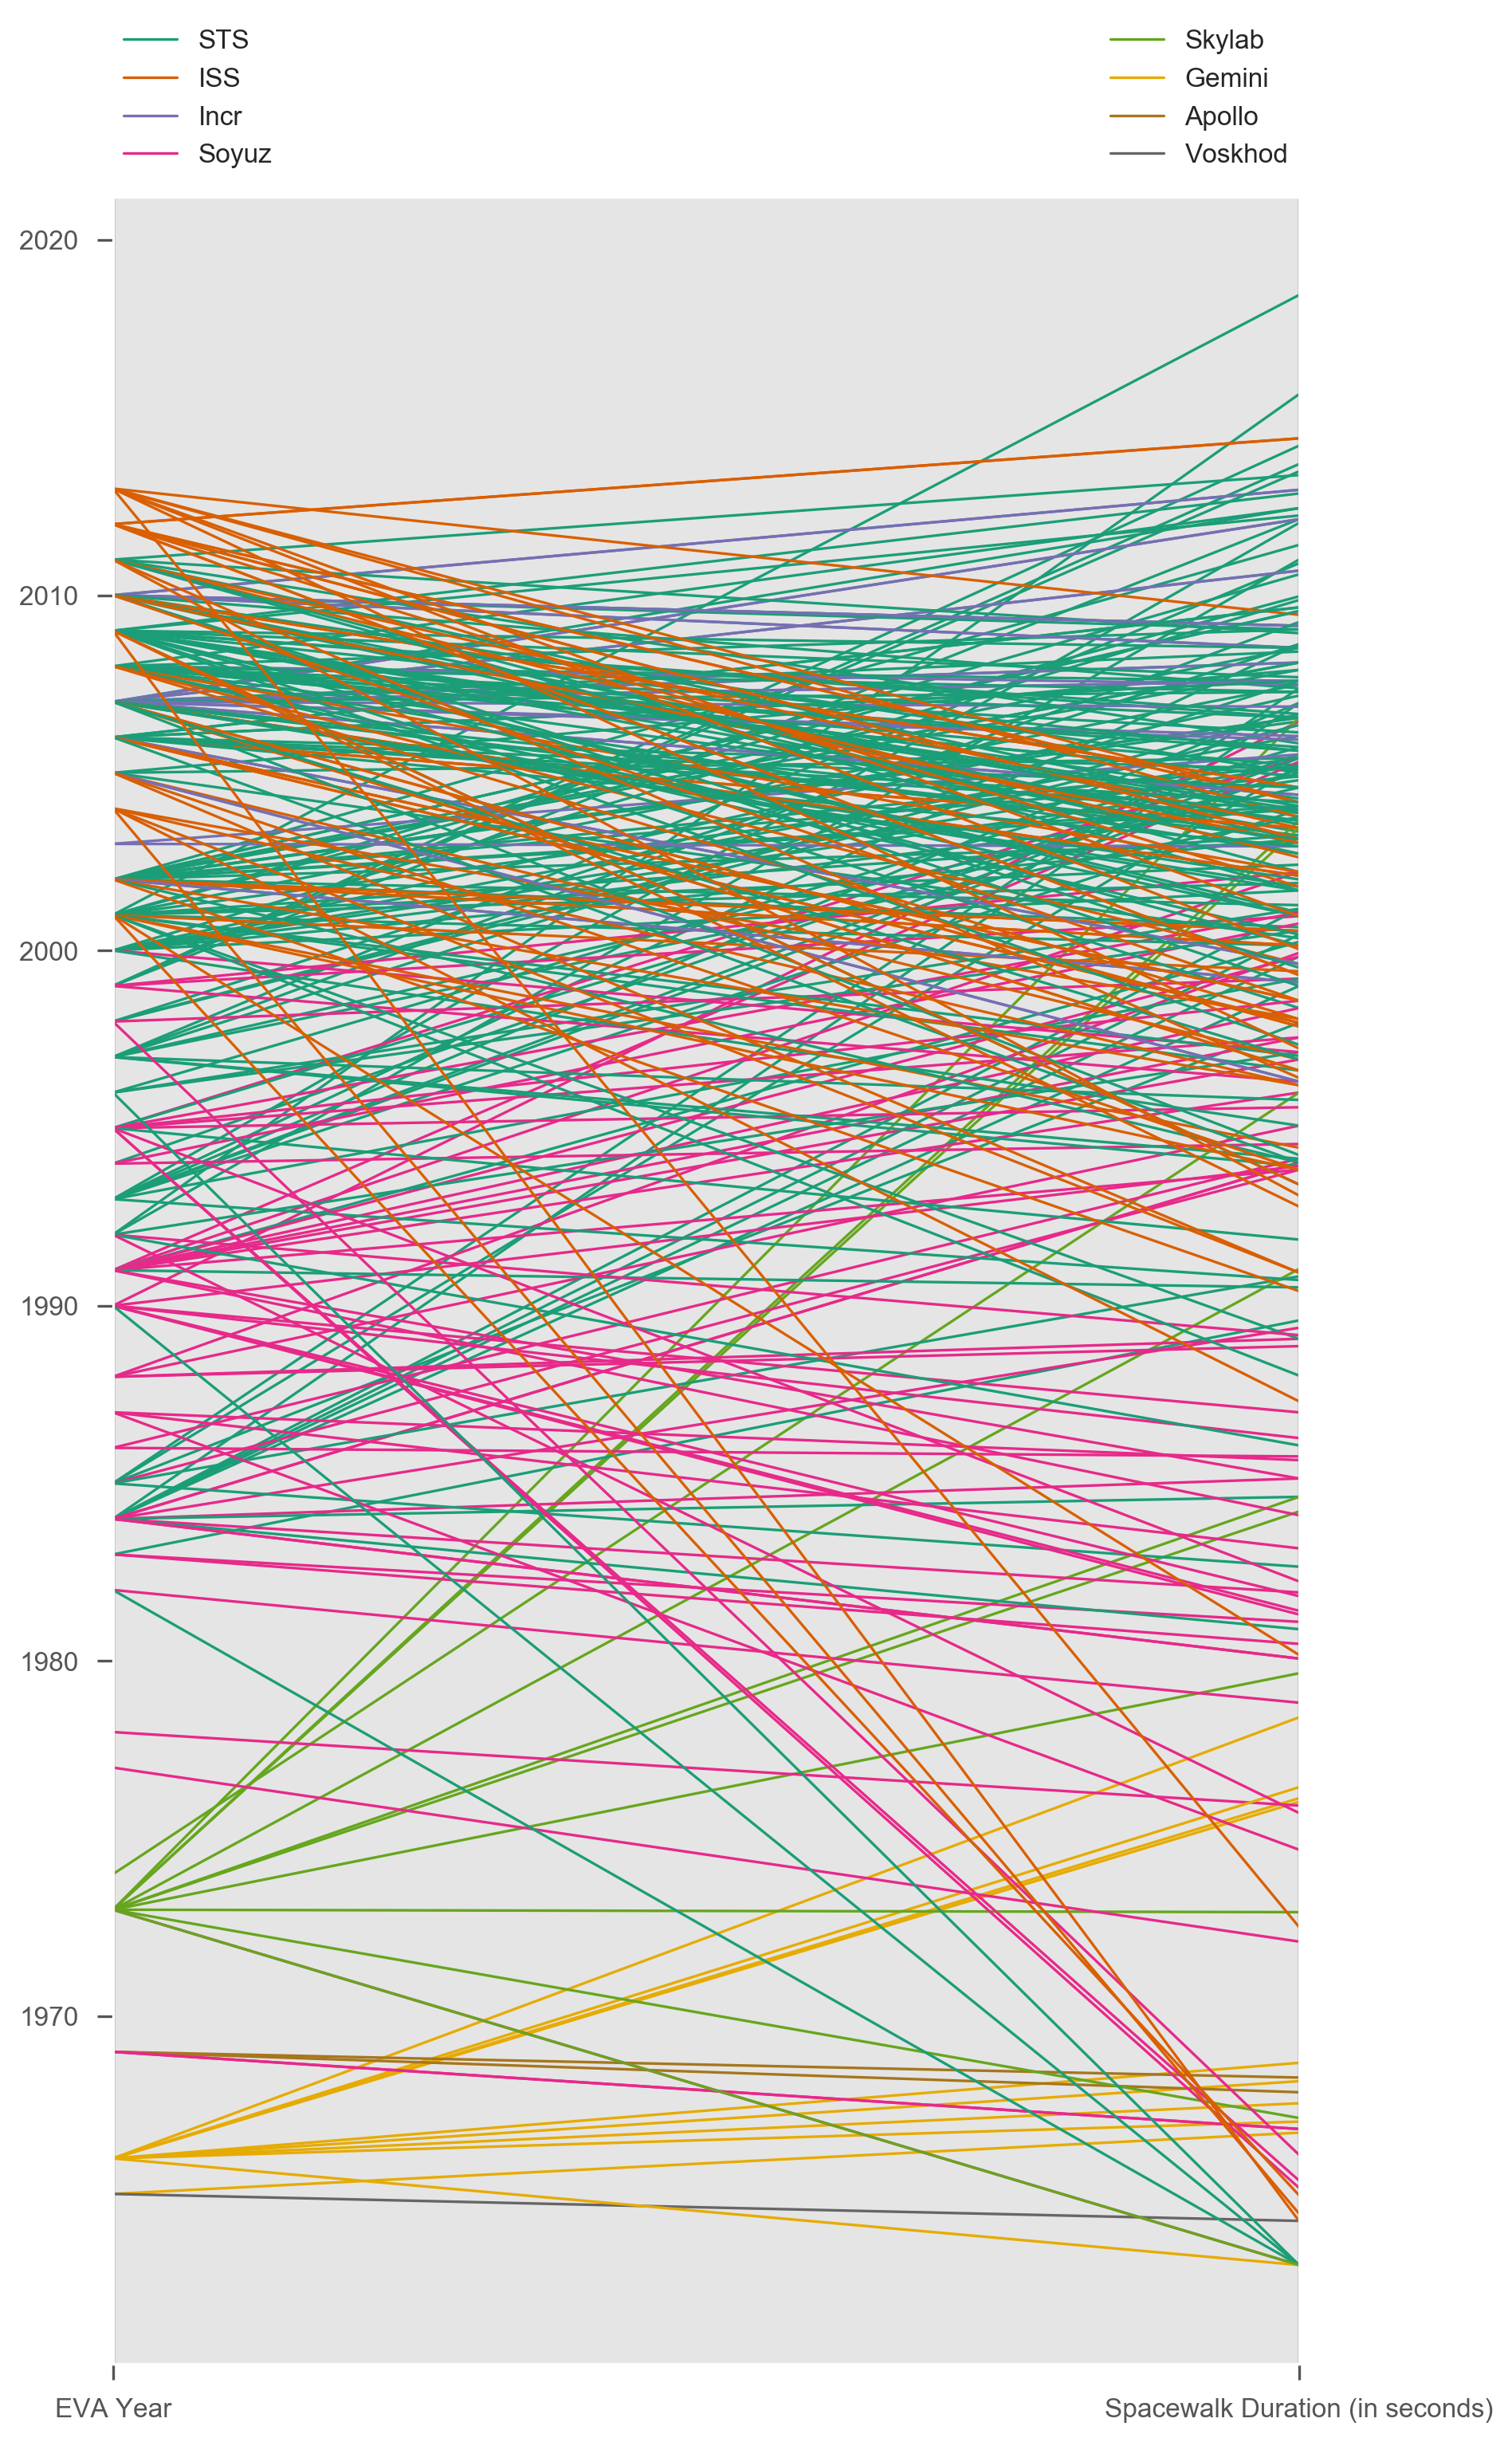
\includegraphics[height=1.0\textheight]{images/fig2.png}
	\caption{Parallel Coordinate Launch Year and EVA}\label{f:fig2}
\end{figure*}


In Figure \ref{f:fig3} we show a scatterplot of mission inclination colored by country of launch. A pattern reflective of launchsites and mission destinations is apparent.

\begin{figure}[p]
	\centering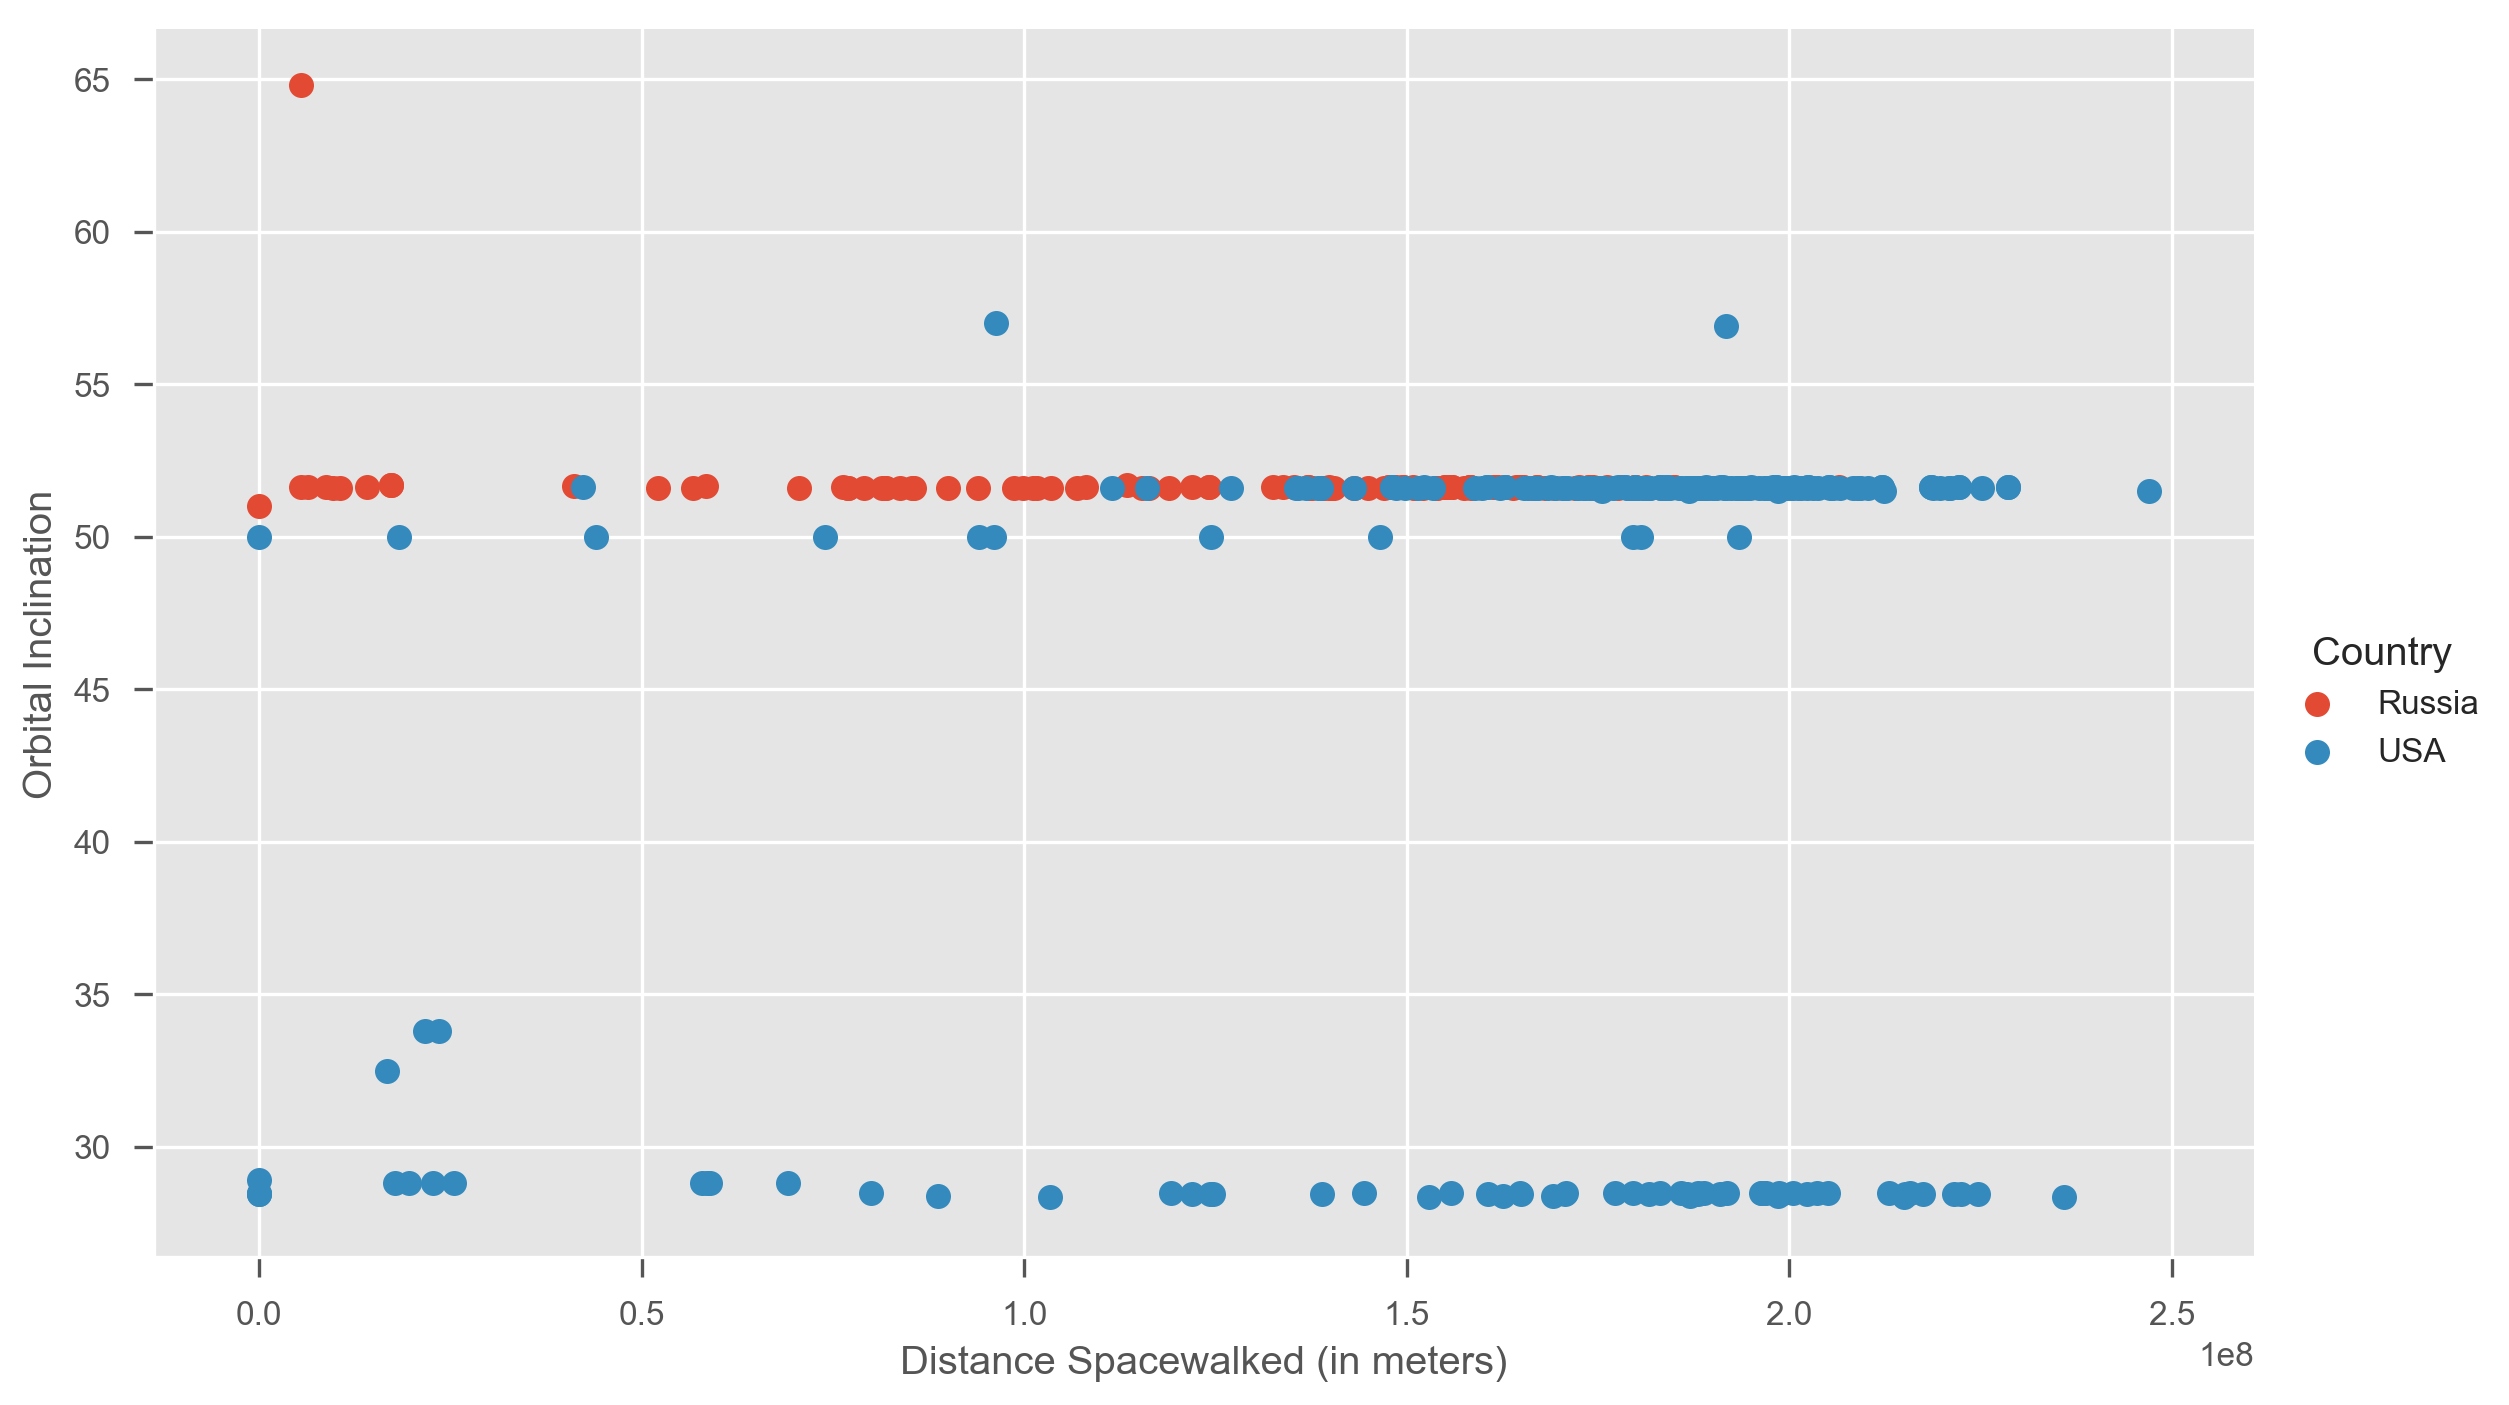
\includegraphics[width=\columnwidth]{images/fig3.png}
	\caption{Inclination and Country}\label{f:fig3}
\end{figure}


In Figure \ref{f:fig4} we show the linear regression results of the reported orbital period versus the predicted period calculated from other fields in the data. 

\begin{figure}[htb]
	\centering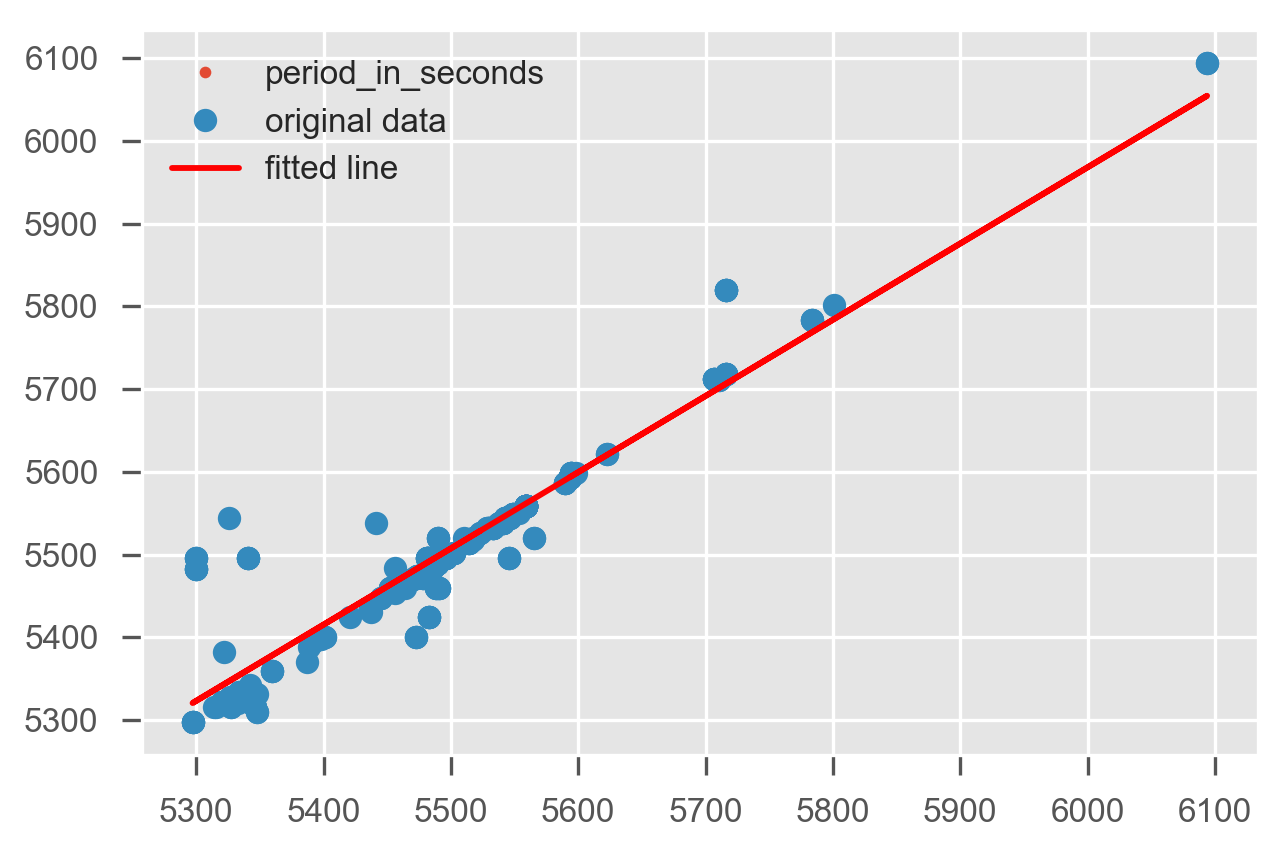
\includegraphics[width=\columnwidth]{images/fig4.png}
	\caption{Linear Regression}\label{f:fig4}
\end{figure}



\section{Tables}

\begin{table*}[htb]
	\centering
	\caption{Table 1. Longest Distance Spacewalks}
	\label{mytable}
\resizebox{\textwidth}{!}{%
	\begin{tabular}{llllllllll}
		\textbf{Vehicle} & \textbf{Date} & \textbf{Duration} & \textbf{Distance Spacewalked (meters)} & \textbf{Crew 1}    & \textbf{Crew 2}      & \textbf{Crew 3} & \textbf{Spacewalk Duration (seconds)} & \textbf{Orbital Perimeter} & \textbf{Orbital Velocity} \\
		STS-102          & 3/10/2001     & 8:56              & 246946540                              & Jim Voss           & Susan Helms          &                 & 32160                                 & 42432.42                   & 7678.69                   \\
		STS-49           & 5/13/1992     & 8:29              & 235881646                              & Pierre J. Thuot    & Richard J. Hieb      & Thomas D. Akers & 30540                                 & 41986.01                   & 7723.70                   \\
		Expedition 32    & 8/30/2012     & 8:17              & 228596876                              & Sunita Williams    & Akihiko Hoshide      &                 & 29820                                 & 42614.69                   & 7665.89                   \\
		STS-134          & 5/22/2011     & 8:07              & 225199861                              & Andrew Feustel     & Mike Fincke          &                 & 29220                                 & 42159.08                   & 7707.05                   \\
		STS-103          & 12/22/1999    & 8:15              & 224675143                              & Steve Smith        & John Grunsfeld       &                 & 29700                                 & 43754.92                   & 7564.82                   \\
		STS-103          & 12/23/1999    & 8:10              & 222405697                              & Mike Foale         & Claude Nicollier     &                 & 29400                                 & 43754.92                   & 7564.82                   \\
		Expedition 24    & 8/7/2010      & 8:03              & 222157527                              & Doug Wheellock     & Tracy Caldwell Dyson &                 & 28980                                 & 42614.69                   & 7665.89                   \\
		STS-103          & 12/24/1999    & 8:08              & 221497919                              & Steve Smith        & John Grunsfeld       &                 & 29280                                 & 43754.92                   & 7564.82                   \\
		STS-122          & 2/11/2008     & 7:58              & 220991575                              & Rex Walheim        & Stan Love            &                 & 28680                                 & 42177.95                   & 7705.42                   \\
		STS-117          & 6/15/2007     & 7:58              & 220876174                              & Danny Olivas       & Jim Reilly           &                 & 28680                                 & 42234.48                   & 7701.40                   \\
		STS-96           & 5/29/1999     & 7:55              & 219611347                              & Tammy Jernigan     & Dan Barry            &                 & 28500                                 & 42165.38                   & 7705.66                   \\
		STS-110          & 4/11/2002     & 7:48              & 218717662                              & Steve Smith        & Rex Walheim          &                 & 28080                                 & 41266.60                   & 7789.09                   \\
		Expedition 14    & 1/31/2007     & 7:55              & 218477900                              & Mike Lopez-Alegria & Sunita Williams      &                 & 28500                                 & 42614.69                   & 7665.89                   \\
		STS-61           & 12/4/1993     & 7:54              & 217400720                              & Story Musgrave     & Jeff Hoffman         &                 & 28440                                 & 42792.17                   & 7644.19                   \\
		STS-125          & 5/17/2009     & 8:02              & 215733575                              & Mike Massimino     & Mike Good            &                 & 28920                                 & 43415.26                   & 7459.67                   \\
		STS-87           & 11/24/1997    & 7:43              & 215075057                              & Winston Scott      & Takao Doi            &                 & 27780                                 & 41807.25                   & 7742.08                   \\
		STS-49           & 5/14/1992     & 7:44              & 215027670                              & Tom Akers          & Kathy Thornton       &                 & 27840                                 & 41986.01                   & 7723.70                   \\
		STS-125          & 5/15/2009     & 7:56              & 213048095                              & Mike Massimino     & Mike Good            &                 & 28560                                 & 43415.26                   & 7459.67                   \\
		STS-100          & 4/24/2001     & 7:40              & 212401275                              & Scott Parazynski   & Chris Hadfield       &                 & 27600                                 & 42290.94                   & 7695.70                   \\
		Expedition 15    & 7/23/2007     & 7:41              & 212038551                              & Clay Anderson      & Fyodor Yurchikhin    &                 & 27660                                 & 42614.69                   & 7665.89                  
\end{tabular}}
\end{table*}

 

\section{Conclusion}
The distances traveled by spacewalkers are closely related, but not directly calculated from, the durations of spacewalks. This calculation required many fields before it could be determined. The inability to ultimately construct a correct ground trace visualization was disappointing, but a great exercise in both python's Basemap library and a for a more accurate understanding of orbital mechanics. The Wikipedia data parsing by category presents an interface through which other data projects may be pursued and something the author will return to in future work. 



\begin{acks}
	
  The author would like to thank Dr. Gregor von Laszewski and his course TAs for their support.
  
\end{acks}

\bibliographystyle{ACM-Reference-Format}
\bibliography{report} 

\appendix

Included in the Appendix are the three Jupyter notebooks used in this project.

\section{Jupyter Notebooks}

\subsection{Jupyter Notebook 1}
	\DONE{1_gathering_wikipedia_infobox_data.ipynb}

\subsection{Jupyter Notebook 2}
	\DONE{2_data_cleaning_and_merging.ipynb}

\subsection{Jupyter Notebook 3}
	\DONE{3_spacewalk_analysis.ipynb}

 \begin{verbatim}/includegraphics[width=\columnwidth]{images/myimage.pdf}\end{verbatim}

re

\end{document}
